\subsection{IRS observations}
\label{sect:irs_obs}

% SPW: Fig 1: label F_nu(8 \micron), etc., not just "8/24".
\begin{figure}
\centering
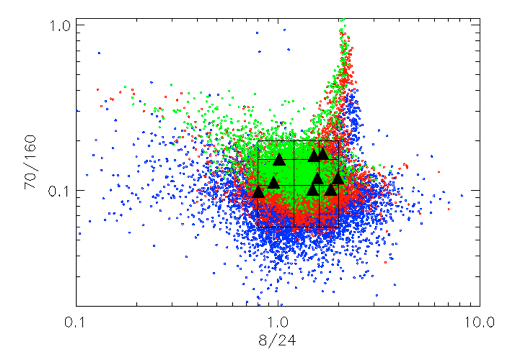
\includegraphics[width = 8 cm]{./colormaps.png}
\caption{$8 - 24/70 - 160$ $\mu$m colour-colour diagram of M31 obtained from IRAC and MIPS. The plot is divided into 9 regions (black grid) and the observations were made to cover those regions. The triangles indicate the regions we observed. ({\bf Needs a better explanation} )}
\label{colourmaps}
\end{figure}

We obtained mid-infrared spectral maps of 12 regions in M31 using the {\em Spitzer}/IRS instrument \citep{IRS2004} covering wavelengths from 5 to 21 microns. 
These regions include the nucleus, two regions previously observed by ISOCAM, and 9 other regions chosen to cover a range of UV intensities, 
metallicities and dust temperatures. Dust temperatures were determined using an $8 - 24/70 - 160$ $\mu$m colour-colour diagram 
(see Figure~\ref{colourmaps}). The locations of the observed regions are shown in Figure~\ref{m31}, and 
their coordinates are given in Table~\ref{regions}. The two regions previously observed by ISOCAM are the region from the bulge and the 
region from the active region in the star-forming ring (Region 9 in our sample). A background observation was also made off the galaxy 
along the minor axis and it was used to enable the background subtraction from the data cubes.

% SPW: Table 1: mark (with a footnote) the regions that have ISO data.
%MLNA: Table 1 would be better if it included the galactocentric radii (perhaps), and the UV intensities, metallicities, and dust temperatures (definitely) used to choose them as targets in the first place.  Also which fields were previously observed by ISO/ISOCAM.  Suggested new title: Spitzer/IRS Target Locations in M31.

%SPW: As to tables, I'd consolidate 1, 2, and 5 into a single table.  Add rows as appropriate for "nucleus" and "north", and give their dimensions in a footnote.  
\begin{table}
 \centering
 \begin{minipage}{70mm}
\caption{IRS Targets and their metallicities in M31
\label{regions}}
  \begin{tabular}{lccc}
  \hline Name & R.A. & Decl. &$12+\log({\rm O/H})$
   \\
 \hline
 Nucleus$^a$&00:42:44.31&41:16:09.4& - - -\\
Bulge$^a$&00:42:35.00&41:21:01.0&$8.90\pm0.03$\\
Region 1&00:41:30.41&40:43:07.8&$9.20\pm0.20$\\
Region 2&00:45:22.85&41:38:53.1&$9.07\pm0.02$\\
Region 3&00:40:37:37&41:01:29.4&$8.85\pm0.01$\\
Region 4&00:41:17.86&41:07:09.8&$8.89\pm0.06$\\
Region 5&00:43:39.57&41:19:03.1&\hspace{0.14cm}$8.93\pm0.08$$^b$\\
Region 6&00:43:35.72&41:23:15.0&$8.73\pm0.08$\\
Region 7&00:40:53.98&40:58:58.9&$8.40\pm0.08$\\
Region 8&00:42:21.60&41:07:17.4&\hspace{0.14cm}$8.94\pm0.08$$^b$\\
Region 9$^a$&00:41:00.00&40:36:20.3&$8.86\pm0.02$\\
NGC206&00:40:20.20&40:44:54.0& - - -\\
Background&00:44:41.8&40:58:56.0& - - -\\
\hline
\end{tabular}
{$^a$Regions that have ISOCAM data. 
$^b$Metallicity values obtained from the radial metallicity profile of M31.}
\end{minipage}
\end{table}

\begin{figure*}
\centering
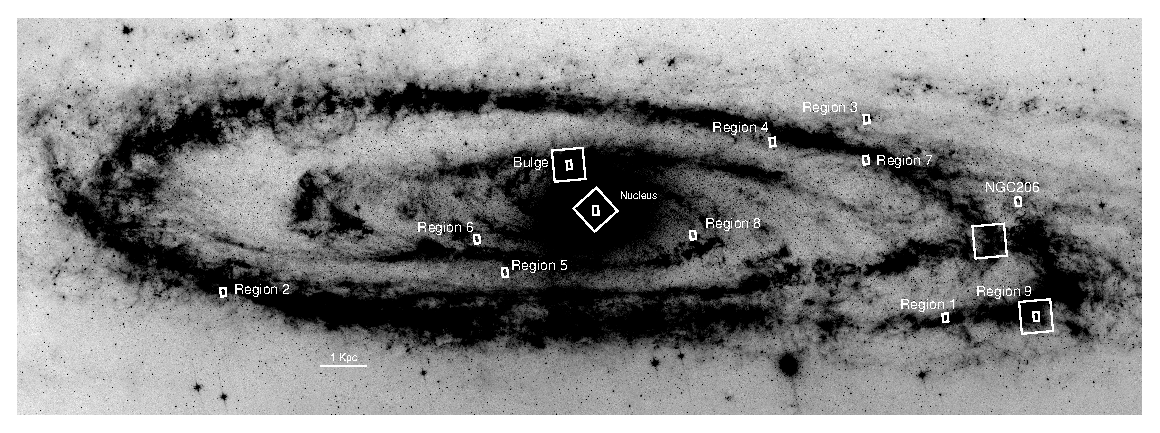
\includegraphics[scale=0.9]{./m31_map.eps}
\caption{An 8 micron IRAC image of M31 \citep{Barmby2006lr}. Small white rectangles ($30\arcsec\times50\arcsec$) show the regions that we observed and larger squares ($192\arcsec\times192\arcsec$) show the regions observed by  \citet{1998Cesarsky}.
\label{m31}
}
\end{figure*}

% SPW: Probably no need to mention LL1, which wasn't used.
For our observations we used the Short-Low (SL) and Long-Low (LL) modules which cover wavelengths from 5 to 21 microns. 
The Low modules have resolving power changing 60--130. Each low-resolution module is divided into two sub-slits 
which provide spectroscopy in either first or second order. They are denoted as SL1 (7.5--14.5~$\mu$m), SL2 (5.2--7.6~$\mu$m),
LL1 (20.5--38.5~$\mu$m), and LL2 (14.5--20.75~$\mu$m).

All regions were observed in September 2007 (PID 40032) with both orders of the Short-Low module (SL2, SL1) and the Long-Low order LL2. 
The Long-Low order LL1 was not used for observations because this spectral region contains few features. The map size was based on the size 
of the IRS slits (SL: $3.6\arcsec \times 57\arcsec$, LL: $10.5\arcsec \times 168\arcsec$). Each region was covered by 18 overlapping observations 
of the SL slit and 11 overlapping observations of the LL slit making the map size $32\arcsec \times 57\arcsec$ for SL and $58\arcsec \times 168\arcsec$ for LL. 
Figure~\ref{slits} shows an example of the slit arrangement. For the brighter regions (nucleus, bulge), ramp times of 14 s (SL) and 30 s (LL) were used, 
while for the fainter regions, ramp times of 60 and 120 s were used respectively. Background observations were taken with each module (2 per ramp time). 
Since all of the targets are in the same part of the sky, a common background observation was used for multiple targets to subtract the background emission. 

% SPW:  I don't really understand this figure or why it's needed.  Is the point that the SL and LL slits don't align?  You could say that in text and omit the figure.  Alternatively, the figure might make sense with a better caption.  Why two SL regions, for example?
\begin{figure}
\centering
\includegraphics[scale=0.3]{./cubeslits.eps}
\caption{SL1 data cube from the nucleus showing the arrangement of slits used to cover the region. 
Black boxes outline the footprints of the SL1 and the green box outlines the LL2. Blue and red slits show how 
each mode was covered using overlapping slit positions.
\label{slits}
}
\end{figure}

\subsection{IRS Data Reduction}

% SPW: it seems obvious, but it might be worth an explicit mention that all the IRS maps cover additional area than is considered here.
The data were reduced through the SSC pipeline (ver. S17.2.0) and the maps were assembled using the CUBISM program \citep{Smith:2007fk}. 
Bad pixel removal was also done using CUBISM and the background observations were used to subtract the background emission from these cubes 
following the method outlined in \citet{Gordon:2008lr}. Spectra were extracted using a $30\arcsec\times50\arcsec$   rectangular aperture. 
The aperture size was selected to cover the whole overlapping area of the SL and LL modes.

After the spectral extraction there was a noticeable mismatch between the spectra from the SL1 and LL2 modules. To combine all spectra to obtain one spectrum, 
first a photometric comparison was conducted between the IRS spectra and the IRAC 8 micron image of M31 \citep{Barmby2006lr}. For more details 
about this method see the IRAC Instrument Handbook Section 4. An aperture with the same size was used to extract flux from the same regions 
in the IRAC 8 micron image. The photometric calibration of the IRAC is tied to point sources measured within a standard aperture with a radius of 12\arcsec. 
For extended sources,  an aperture correction has to be conducted as mentioned in the IRAC instrument handbook. Therefore an extended source 
aperture correction of 0.824 was applied for all the extractions from the 8 $\mu$m image. The uncertainty value of the IRAC image was estimated 
by taking the standard deviation of pixels values within an aperture of the same size from a position off M31 (00:48:58.00, +42:14:54.00).

% SPW: the color correction factor needs a bit of explanation. Isn't it simply the actual IRS spectrum integrated over the IRAC band's responsivity?  The key thing in the IRAC handbook should be the responsivity curves, not the method.  Just which data did you integrate?  I'd have expected it to be SL2 because otherwise the break between SL1 and SL2 is in the middle of the IRAC filter.  Anyway, some clarification is needed here about exactly what you did.
Then we stitched the SL1 and SL2 using the overlapping regions and applied a colour correction factor $K$, which is a multiplicative factor that 
converts the intensity of an IRS spectrum at a given wavelength to the intensity of an IRAC image taken at the same wavelength. We used the IDL 
code provided by the instrument handbook to compute these $K$ values for all the regions. colour correction values and the corresponding IRS 
data along with the IRAC data are given in Table~\ref{colourK}.

% SPW: Table 2: headers should clarify the difference between IRS specific intensity measured at 8.00 microns (if that's what it is) and IRAC specific intensity measured over the broader bandwidth.  I'd suggest "at 8.00~\micron" for the former and "in 8~\micron\ band" for the latter, but perhaps you can do better.  Using footnotes might be a good alternative.
%
%MLNA: Table 2 should make explicit that the fluxes given are prior to color-correction

\begin{table}
 \centering
 \begin{minipage}{90mm}
\caption{Matched aperture photometry}
  \begin{tabular}{lcccc}
  \hline{Name}&{IRS Intensity}&{IRAC Intensity}&{colour K$^b$}&{x$^{a,}$ $^c$} \\ {}&{at 8 $\mu$m$^a$}&{at 8 $\mu$m$^a$}&{}&{} 
   \\
 \hline
 Region 1 & 1.8505 & 1.3923 & 0.532 & 0.3061
 \\ Region 2  & 1.8238 & 1.3731 & 0.555 & 0.2148
 \\ Region 3 & 0.7192 & 0.9689 & 0.767 & 0.3218
 \\ Region 4 & 1.1431 & 0.8513 & 0.589 & 0.0407
 \\  Region 5 & 0.6787 & 0.8088 & 0.773 & 0.1834
 \\  Region 6  & 0.6399 & 0.7656 & 0.927 & 0.0479
 \\  Region 7  & 1.1538 & 0.8243 & 0.526 & 0.1380
 \\ Region 8 & 0.5556 & 0.7135 & 0.877 & 0.1148
 \\  Region 9 & 1.9413 & 1.6562 & 0.606 & 0.3107 
 \\ Bulge & 2.6956 & 2.5473 & 0.532 & 1.2425\\
\hline
 \label{colourK}
\end{tabular}\\
 {$^a$Units are MJy~sr$^{-1}$. 
 $^b$Colour correction factors 
 $^c$Offset between IRAC and IRS as mentioned in eq. 1. Intensities are given prior to the extended source correction and the colour correction.}
\end{minipage}
\end{table}

% SPW: it isn't clear to me exactly how you estimated the IRAC uncertainty.
%Eq 1: because the IRAC uncertainties are much smaller than the IRS ones, you have to use the IRAC intensities as the independent variable (unless you take uncertainties on both axes into account in the fitting).  This probably won't change the answer much, but it might.

%MLNA: How was the line of best fit derived -- did you weight by uncertainty?
%
Figure~\ref{offset} compares the IRS and IRAC 8~$\mu$m photometry. The line of best fit wighted by the uncertainties has a slope of $0.81\pm0.08$ 
and intercept of $-0.05\pm0.06$.  Since the intercept in Figure~\ref{offset} is not zero with a higher uncertainty, it can be concluded that the offsets 
between orders are due to an additive offset than a multiplicative offset. Also an additive offset favours more for stitching SL and LL modes. 
Based on this argument, first we shifted the combined SL1 and SL2 spectrum so that the intensity at 8 $\mu$m matches with that of IRAC 8 micron image. 
To do this shift, the following equation was used to find the offset values ($x$) between IRS and IRAC image intensities at 8 microns. 
\begin{equation}
F_{IRAC8} = [ F_{IRS8} + x ] \times K
%K is the colour correction factor.
\end{equation}
\footnotesize
%\emph{Where K is the colour correction factor, Flux$_{IRAC8}$ is the flux of the IRAC 8 $\mu$m image, Flux$_{IRS8}$ is the flux of IRS spectra at 8 $\mu$m and x is the offset.}
\normalsize
$K$ is the colour correction factor, F$_{IRAC8}$ is the intensity of the IRAC 8 $\mu$m image (aperture corrected) and F$_{IRS8}$ is the intensity of IRS spectra at 8~$\mu$m. 
The offsets for all the regions are listed in Table \ref{colourK}. After that the LL2 mode was stitched by shifting it towards the SL1 by an amount of the average difference in their overlapping spectral regions.	
% SPW: Sec 2.2 par 5: clarify that "stitched to" means via an additive constant for each spectrum.
%MLNA Can you cite others who applied *offsets* to force IRS spectra to match up, as opposed to using only multiplicative factors -- is this standard practice?
%

	
\begin{figure}
\centering
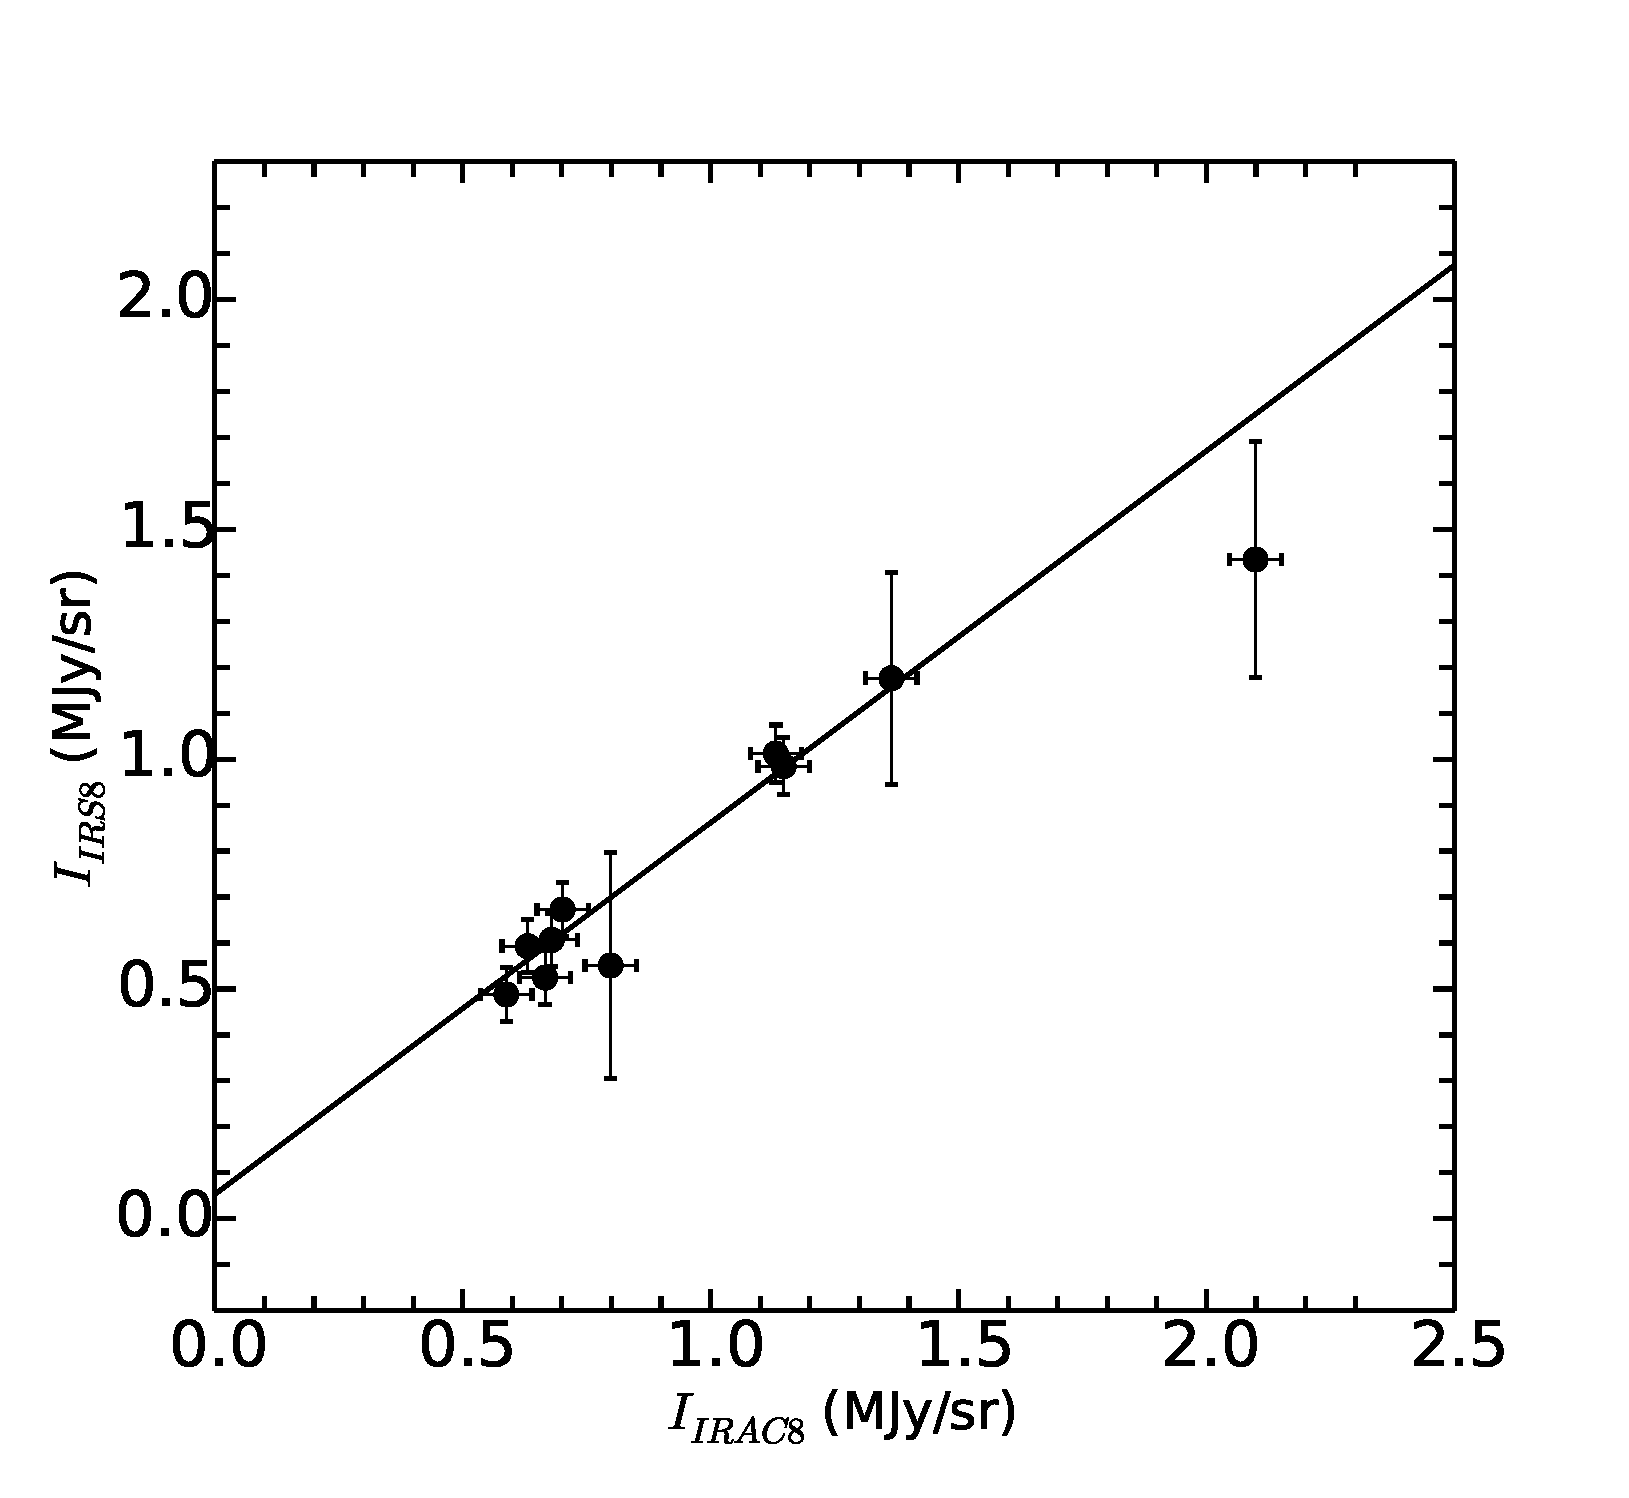
\includegraphics[scale=0.25]{./offset.eps}
\caption{ Intensity of the aperture corrected IRAC 8~$\mu$m image vs that of the colour corrected IRS spectra at 8~$\mu$m  obtained using the same aperture for our regions in M31. The straight line is the line of best fit. }
\label{offset}
\end{figure}

% TODO: tables need some reformatting, such as $x\pm y$

\begin{table*}
 \centering
 \begin{minipage}{200mm}
\caption{PAH Emission Line Strengths$^a$}
  \begin{tabular}{l c c  c  c  c  c  c  c  c  c c }
  \hline {Region  }&{5.7$\mu$m  }&{6.2$\mu$m  }&{7.7$\mu$m  }&{8.3$\mu$m  }&{8.6$\mu$m  }&{10.7$\mu$m  }&{11.3$\mu$m  }&{12.0$\mu$m  }&{12.7$\mu$m  }&{17.0$\mu$m  } 
   \\
 \hline
 Region 1 &$10\pm1$            & $34\pm1$        & $107\pm10$        & $13\pm1$       & $14.1\pm0.9$        & $2.2\pm0.3$        & $33.4\pm0.9$        & $9.1\pm0.5$        & $16\pm1$        & $17\pm1$        \\
Region 2 &$7.7\pm0.9$        & $31.2\pm0.8$        & $106\pm8$        & $9\pm1$           & $19.8\pm0.8$        & $1.5\pm0.2$        & $32.0\pm0.8$        & $6.6\pm0.4$        & $15\pm1$        & $14.7\pm0.9$        \\
Region 3 &$8\pm4$              & $25\pm3$                & $111\pm22$       &$21\pm4$       & $7\pm3$                 & $1.1\pm0.9$        & $19\pm3$             & $6\pm1$             & $14\pm3$           & $13\pm2$        \\
Region 4 &$4\pm1$              & $15.8\pm0.9$        & $59\pm9$        & $7\pm1$           & $11.6\pm0.8$          & $0.8\pm0.2$        & $19.9\pm0.8$        & $3.5\pm0.4$        & $9\pm1$             & $12.5\pm0.9$        \\
Region 5 &$1\pm1$              & $7\pm1$                 & $22\pm3$        & $3\pm1$           & $5.8\pm0.8$            & $0.9\pm0.2$        & $12.7\pm0.8$        & $2.4\pm0.4$        & $6.3\pm0.4$        & $10\pm2$        \\
Region 6 & - - - -                      &$ 7.3\pm0.9$         & $22\pm7$        & $3\pm1$            & $3.6\pm0.8$       & $0.8\pm0.2$        & $10.8\pm0.8$        & $1.9\pm0.4$        & $4.5\pm0.4$        & $8.3\pm0.6$        \\
Region 7 &$5.9\pm0.9$        & $17.7\pm0.9$       & $57\pm8$        & $9\pm1$            & $12.8\pm0.8$        & $1.6\pm0.2$        & $21.8\pm0.8$        & $5.2\pm0.4$        & $11\pm1$             & $13\pm2$        \\
Region 8 &$2.\pm1$              & $3\pm1$              & $6\pm3$            & $3\pm1$            & $2.7\pm0.8$        & $1.4\pm0.3$        & $4.4\pm0.8$            & - - - -                      &  - - - -               & $4.1\pm0.7$        \\
Region 9 &  - - - -                     & $38\pm3$          & $133\pm29$        & $25\pm4$        & $15\pm3$            & $2.4\pm0.8$        & $37\pm3$               & $14\pm1$             & $25\pm3$        & $19\pm6$        \\
Bulge       & - - - -                       & $38\pm2$           & $219\pm27$        & $32\pm4$        & $20\pm3$           & $2.0\pm0.9$        & $53\pm3$              & $14\pm1$           & $29\pm3$        & $39\pm2$       \\
\hline
 \label{PAHlinetable}
\end{tabular}\\
{$^a$Units are 10$^{-9}$~W~m$^{-2}$.}
\end{minipage}
\end{table*}







\begin{table*}
 \centering
 \begin{minipage}{200mm}
\caption{PAH Emission Line Equivalent Widths$^a$}
  \begin{tabular}{l c c  c  c  c  c  c  c  c  c c }
  \hline {Name  }&{5.7$\mu$m  }&{6.2$\mu$m  }&{7.7$\mu$m  }&{8.3$\mu$m  }&{8.6$\mu$m  }&{10.7$\mu$m  }&{11.3$\mu$m  }&{12.0$\mu$m  }&{12.7$\mu$m  }&{17.0$\mu$m  } 
   \\
 \hline
 Region 1 &$0.39\pm0.08$        & $1.2\pm0.1$             & $3.4\pm0.3$        & $0.43\pm0.04$        & $0.47\pm0.04$        & $0.09\pm0.01$        & $1.45\pm0.04$        & $0.43\pm0.03$        & $0.78\pm0.03$              & $1.27\pm0.05$        \\
 Region 2 &$0.28\pm0.04$        & $1.02\pm0.06$        & $3.4\pm0.2$        & $0.32\pm0.04$        & $0.70\pm0.04$        & $0.07\pm0.01$        & $1.58\pm0.04$        & $0.35\pm0.02$        & $0.85\pm0.03$              & $1.35\pm0.06$        \\
 Region 3$^b$ &$4\pm2$           & $8\pm2$                   & $19\pm4$            & $2.8\pm0.8$             & $0.9\pm0.5$             & $0.1\pm0.1$            & $2.1\pm0.3$             & $0.7\pm0.2$            & $1.6\pm0.2$                   & $2.4\pm0.3$        \\
 Region 4 &$0.28\pm0.09$        & $1.0\pm0.1$             & $3.7\pm0.4$       & $0.5\pm0.1$              & $0.77\pm0.07$        & $0.07\pm0.02$        & $1.67\pm0.06$        & $0.31\pm0.04$        & $0.86\pm0.05$             & $1.68\pm0.07$        \\
 Region 5 & - - - -                          & $0.12\pm0.03$        & $0.61\pm0.08$   & $0.10\pm0.03$        & $0.20\pm0.03$        & $0.05\pm0.01$        & $0.77\pm0.03$        & $0.17\pm0.03$        & $0.50\pm0.04$            & $1.6\pm0.2$        \\
 Region 6 & - - - -                          & $0.10\pm0.04$        & $0.6\pm0.2$        & $0.10\pm0.04$        & $0.14\pm0.03$        & $0.05\pm0.01$        & $0.77\pm0.04$        & $0.15\pm0.03$        & $0.42\pm0.04$            & $1.7\pm0.1$        \\
 Region 7 &$0.32\pm0.05$        & $0.86\pm0.06$        & $2.8\pm0.2$        & $0.44\pm0.06$        & $0.69\pm0.06$        & $0.12\pm0.02$        & $1.81\pm0.07$        & $0.48\pm0.05$        & $1.11\pm0.08$            & $2.2\pm0.2$        \\
 Region 8 &$0.03\pm0.04$        & $0.04\pm0.03$        & $0.2\pm0.10$      & $0.09\pm0.04$        & $0.10\pm0.03$        & $0.09\pm0.02$        & $0.30\pm0.02$        & $0.00\pm0.00$        & $0.01\pm0.01$            & $0.62\pm0.07$        \\
 Region 9$^b$ & - - - -                 & $237\pm100$          & $151\pm60$        & $16\pm6$                 & $8\pm3$                   & $0.5\pm0.2$             & $7\pm1$                   & $2.3\pm0.6$             & $3.6\pm0.8$                 & $2.4\pm0.8$  \\
 Bulge       & - - - -                          & $1.2\pm0.2$            & $4.0\pm0.4$        & $0.51\pm0.07$         & $0.30\pm0.06$        & $0.03\pm0.01$        & $0.78\pm0.03$        & $0.22\pm0.02$        & $0.49\pm0.03$            & $1.16\pm0.04$ \\             
\hline
 \label{EQW}
\end{tabular}\\
{$^a$Units are $\mu$m.
%SPW Table 3: fn b _probably_ should be something like "Continuum for these regions is very weak.  Equivalent widths are highly uncertain and not considered in the analysis."
 
$^b$EQWs from these two regions were removed from the analysis (see Section~\ref{sect:data_analysis}).}
\end{minipage}
\end{table*}





%MLNA: Table 5 has names inconsistent with other tables in the paper
% PB: fixed?
\begin{table*}
 \centering
 \begin{minipage}{100mm}
\caption{Atomic Emission Line Strengths$^a$}
  \begin{tabular}{l c c  c  c  c  c  }
  \hline{Name  }&{[Ar~{\sc ii}] }&{[Ar~{\sc iii}]  }&{[S~{\sc iv}]}&{[Ne~{\sc ii}]   }&{[Ne~{\sc iii}]   }&{[S~{\sc iii}]  }\\
{}&{\tiny{7.0$\mu$m} }&{\tiny{9.0$\mu$m }}&{\tiny{10.5$\mu$m}}&{\tiny{12.8$\mu$m  }}&{\tiny{15.5$\mu$m } }&{\tiny{18.7$\mu$m }} 
   \\
 \hline 
 
Region 1 &    $<$15.2                 & $<$16.4                 & $6\pm1$                 & $6\pm1$                 & $<$ 4.2                 & $2.2\pm0.4$                \\
Region 2 &    $5\pm3$                 & $<$ 17.4               & $<$5.1                    & $6\pm1$                 & $<$ 2.9                 & $0.9\pm0.5$                 \\
Region 3 &    $<$42.9                 & $27\pm6$              & $<$ 28.9                & $9\pm3$                 & $6\pm1$               & $4.3\pm0.9$                 \\
Region 4 &    $<$11.2                 & $<$10.0                 & $<$4.4                    & $2\pm1$                 & $0.6\pm0.5$        & $1.3\pm0.5$                 \\
Region 5 &    $4\pm3$                 & $<$6.2                   & $<$ 5.2                 & $<$ 4.2                     & $2\pm1$               & $2\pm1$                 \\
Region 6 &    $7\pm3$                & $4\pm2$                 & $<$ 3.8                 & $2\pm1$                  & $5.4\pm0.5$         & $5.3\pm0.5$                 \\
Region 7 &    $3\pm3$                 & $<$12.6                 & $2.3\pm0.9$        & $10\pm2$                & $<$ 2.9                 & $8\pm1$                \\
Region 8 &    $<$11.8                  & $5\pm2$                & $<$4.9                  & $<$2.6                      & $11.6\pm0.5$     & $6.5\pm0.5$                 \\
Region 9 &    $24\pm10$             & $35\pm8$             & $<$ 2.7                 & $38\pm3$                 & $7\pm4$               & $15.3\pm5.6$                 \\
Bulge &          $10\pm7$               & $49\pm7$              & $<$ 30.4               & $19\pm4$                 & $7\pm2$               & $2\pm1$      \\            

\hline
 \label{Atomic}
\end{tabular}\\
{ $^a$Units are 10$^{-10}$~W~m$^{-2}$. Upper limits are indicated with a $<$ mark.  }
%SPW: Table 4: units of 10^-10 W m^-2 must be wrong.  I'd expect 10^-15 or so.
%How many sigma are the upper limits?

\end{minipage}
\end{table*}



\subsection{ISOCAM Data Reduction}

% SPW:  mention ISO spectral resolution.  I would have preferred to see the ISO FOV and wavelength range mentioned earlier, but I don't see any good place to put them other than here, though the Fig 2 caption is a possibility for the FOV.  Another is a footnote where ISOCAM is mentioned in Sec 2.1 par 1, though I'm not sure ISOCAM should really appear there at all.

To compare our results with previous observations, ISOCAM data of three regions previously observed by \citet{1998Cesarsky} which overlap 
with IRS observations were obtained. We retrieved the highly processed data provided by \citet{Boulanger_F_2005} of these ISOCAM observations. 
The total wavelength range covered was 5.15 to 16.5 $\mu$m and the field-of-view was $32\times 32$ pixels with 6\arcsec\ per pixel. 
An image of the ISOCAM data is shown in Figure~\ref{isonuc}.  For the three regions in common, we extracted spectra using the same aperture as for the IRS data. 

% SPW: Fig 5: mention "negative image" (if that's what it is).  Also mention spectral band of image and the 30x50 box size.
\begin{figure}
\centering
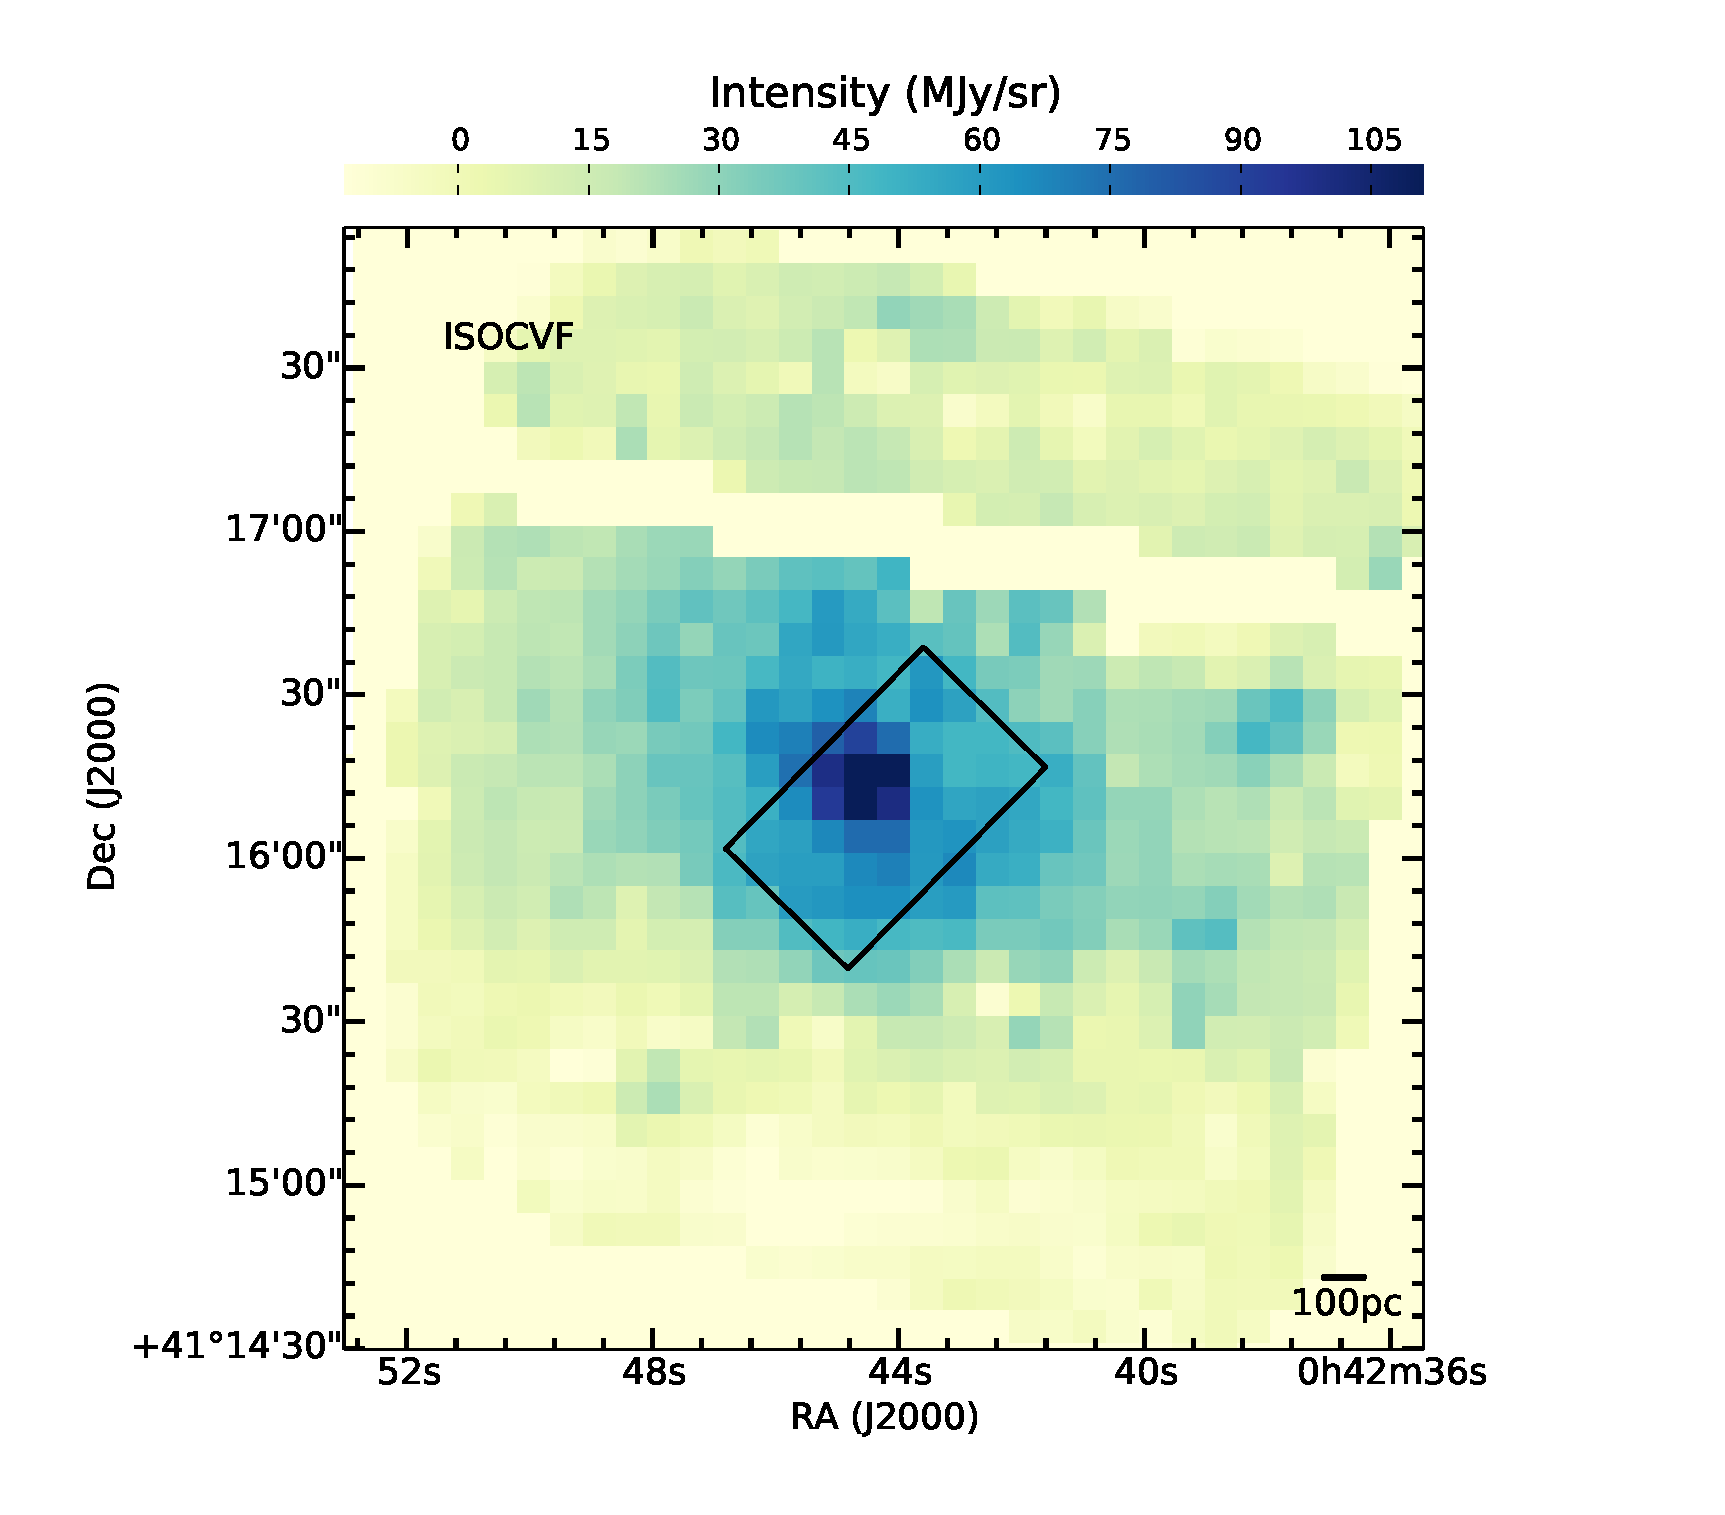
\includegraphics[width = 8cm]{./isonuc.eps}
\caption{11.3~$\mu$m image of the ISOCAM data cube from the nucleus of M31. The black box shows the size of the aperture used to extract spectra.}
\label{isonuc}
\end{figure}
